\chapter{Các khái niệm cơ bản}

\section{Thông tin}

\textbf{- Thông tin:} là cái mà con người trao đổi với nhau

\noindent\textbf{Ví dụ:}

+ Âm thanh

+ Hình ảnh

+ Dữ liệu

\section{Tín hiệu truyền}
- Tín hiệu truyền có 2 loại: \textcolor{red}{digital signal} và \textcolor{red}{analag signal}.

\subsection{Analog signal}
\textbf{- Định nghĩa: }\textcolor{red}{Tín hiệu tương tự} là tín hiệu có biên độ thay đổi theo thời gian.
\begin{center}
    % Vẽ lại tín hiệu và các chú thích trong hình mẫu.
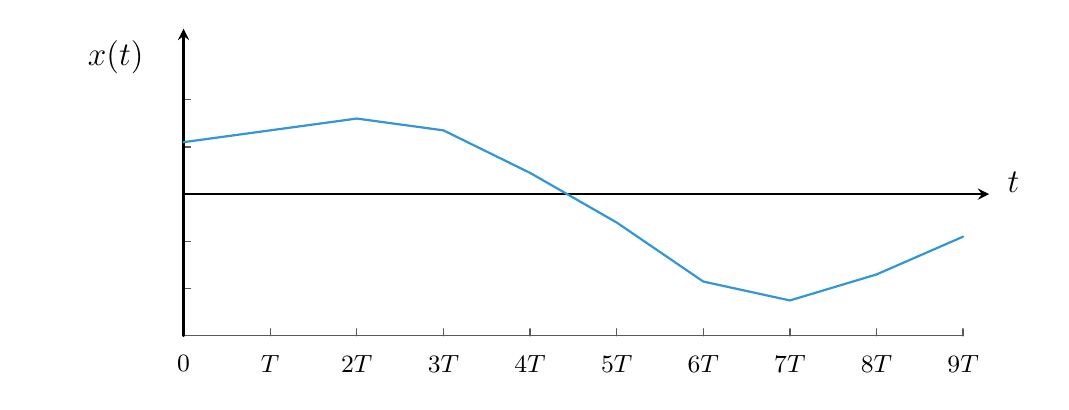
\begin{tikzpicture}[
    x=1.1cm,
    y=6cm,
    font=\small,
    line cap=round,
    line join=round
]
    % Cùng bề rộng với hình lấy mẫu để các mốc thời gian thẳng hàng.
    \path (-1.8, 0) -- (9.9, 0);
    \definecolor{analogsignal}{RGB}{50, 150, 215}

    % Đường chuẩn phía dưới và các vạch chia.
    \draw[black!65, line width=0.45pt] (0, -0.3) -- (9, -0.3);
    \foreach \position in {0,...,9} {
        \draw[black!65, line width=0.45pt]
            (\position, -0.3) -- (\position, -0.285);
    }
    \foreach \level in {-0.3, -0.2, -0.1, 0, 0.1, 0.2} {
        \draw[black!65, line width=0.45pt]
            (0, \level) -- (0.08, \level);
    }

    % Trục biên độ và trục thời gian.
    \draw[->, >=stealth, line width=0.8pt] (0, -0.3) -- (0, 0.35);
    \draw[->, >=stealth, line width=0.8pt] (0, 0) -- (9.3, 0);
    \node[anchor=east, font=\large] at (-0.35, 0.29) {$x(t)$};
    \node[anchor=west, font=\large] at (9.4, 0.025) {$t$};

    % Mốc thời gian theo các chú thích viết tay trên hình mẫu.
    \node[anchor=north] at (0, -0.32) {$0$};
    \node[anchor=north] at (1, -0.32) {$T$};
    \foreach \position in {2,...,9} {
        \node[anchor=north] at (\position, -0.32) {$\position T$};
    }

    % Các điểm biên độ được ước lượng từ ảnh, nối bằng đoạn thẳng.
    \draw[analogsignal, line width=0.8pt]
        (0, 0.11) -- (1, 0.135) -- (2, 0.16) -- (3, 0.135)
        -- (4, 0.045) -- (5, -0.06) -- (6, -0.185)
        -- (7, -0.225) -- (8, -0.17) -- (9, -0.09);

\end{tikzpicture}

\end{center}

\newpage
- Có hai tham số đặc trưng: 

\hspace*{1cm}+ Biên độ (cường độ) - Voltage (V)

\hspace*{1cm}+ Dải tần

\hspace*{2cm}
$
\begin{aligned}
    &\boxed{W = |f_{min} - f_{max}|}\\[6pt]
    &\boxed{B = f_{max} - f_{min}} \text{ - Băng thông (độ rộng băng thông)}
\end{aligned}
$

\noindent\textbf{Ví dụ: } Âm thanh mà con người nghe được là từ $16 - 20000$ (Hz)

\noindent\textbf{Ví dụ: } Âm thanh thoại từ $300 - 3400$ (Hz)

\noindent\textbf{Ví dụ: } Băng thông một kênh truyền hình tương tự: $0 - 6.5$ (MHz)

\subsection{Digital signal}
\begin{center}
    % Tín hiệu số với dãy bit 0 1 0 0 1 0 1 1, vẽ lại từ hình mẫu.
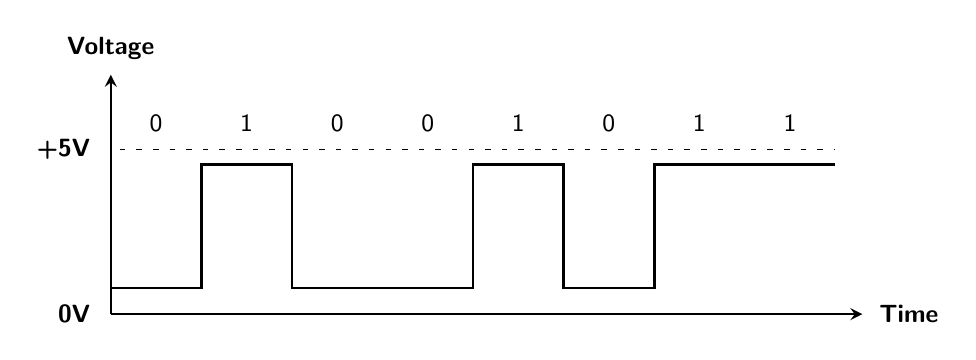
\begin{tikzpicture}[x=1.15cm, y=0.95cm, font=\sffamily\small]
    % Trục điện áp và thời gian.
    \draw[->, >=stealth, line width=0.9pt] (0, 0) -- (0, 3.2);
    \draw[->, >=stealth, line width=0.9pt] (0, 0) -- (8.3, 0);
    \node[anchor=south, font=\sffamily\small\bfseries]
        at (0, 3.28) {Voltage};
    \node[anchor=west, font=\sffamily\small\bfseries]
        at (8.38, 0) {Time};

    % Mức điện áp tham chiếu, giữ cách trình bày của hình mẫu.
    \draw[dash pattern=on 2pt off 4pt, line width=0.6pt]
        (0.1, 2.2) -- (8, 2.2);
    \node[anchor=east, font=\sffamily\small\bfseries]
        at (-0.12, 2.2) {+5V};
    \node[anchor=east, font=\sffamily\small\bfseries]
        at (-0.12, 0) {0V};

    % Các khoảng bit có độ dài bằng nhau.
    \foreach \position/\bit in {0.5/0, 1.5/1, 2.5/0, 3.5/0,
                                4.5/1, 5.5/0, 6.5/1, 7.5/1} {
        \node at (\position, 2.55) {\bit};
    }

    % Xung vuông: các bit liên tiếp cùng giá trị giữ nguyên mức.
    \draw[line width=1pt, line join=miter, line cap=butt]
        (0, 0.35) -- (1, 0.35)
        -- (1, 2) -- (2, 2)
        -- (2, 0.35) -- (4, 0.35)
        -- (4, 2) -- (5, 2)
        -- (5, 0.35) -- (6, 0.35)
        -- (6, 2) -- (8, 2);
\end{tikzpicture}

\end{center}

\textbf{- Định nghĩa: }\textcolor{red}{Digital signal} là tín hiệu có biên độ thay đổi rời rạc theo thời gian

- Có hai tham số đặc trưng:

\hspace*{1cm}+ Tối thiểu hai mức

\hspace*{1cm}+ Tốc độ truyền: $bit/s$, $b/s$, $bps$

\section{Ví dụ tín hiệu 2 mức}
$t_b$: Thời gian truyền 1 bit

$
    \begin{aligned}
        \boxed{v_b = \dfrac{1}{t_b} \quad (bit/s)} \quad \text{Tốc độ bit}
    \end{aligned}
$

Bit 0 = 0V

Bit 1 = 1V

\noindent\textbf{Ví dụ:} Download 1 file kích thước 1 GB từ internet về mất 5 phút. Tính tốc độ download?

\begin{center}
    \textbf{Giải}
\end{center}

1 GB = $1024$ MB

5 phút = 300 giây

$\rightarrow v_b = \dfrac{1024}{300} = 3.41$ MB/s $= 27.3$ Mb/s

\section{Ví dụ tín hiệu 4 mức}
1 mức = 2 bit

\noindent\hspace*{1.5cm} 00 = -3V

\noindent\hspace*{1.5cm} 01 = -1V

\noindent\hspace*{1.5cm} 10 = 1V

\noindent\hspace*{1.5cm} 11 = 3V

\noindent\textbf{Ví dụ: }Cho tín hiệu 4 mức với các mức như bên cạnh. Vẽ tín hiệu 4 mức cho dòng bit.

\begin{center}
    % Khung bài tập tín hiệu 4 mức, vẽ lại từ hình mẫu.
% Dùng trong tài liệu đã nạp gói tikz bằng lệnh \input{...}.
\begin{tikzpicture}[
    x=1.5cm,
    y=0.6cm,
    font=\small\bfseries\boldmath,
    line width=1.1pt,
    line cap=round
]
    \begin{scope}[draw=black, text=black]
        % Sáu vạch chia tạo thành năm khoảng ký hiệu, mỗi khoảng hai bit.
        \foreach \boundary in {0,...,5} {
            \draw (\boundary, -3.6) -- (\boundary, 3.6);
        }

        % Đường ngang ở giữa khung.
        \draw (0, 0) -- (5.85, 0);

        \node[anchor=east] at (-0.45, 3.6) {$S_t=$};
        \node[anchor=east, align=left] at (-0.45, 0)
            {Tín hiệu 4\\mức};

        % Giữ nguyên thứ tự các cặp bit trong ảnh.
        \foreach \position/\bits in {
            0.5/{1\,0},
            1.5/{0\,1},
            2.5/{1\,1},
            3.5/{0\,0},
            4.5/{0\,1}
        } {
            \node at (\position, 3.05) {$\bits$};
        }

        % Bốn mức biên độ; hoàn chỉnh các nhãn bị cắt ở mép ảnh.
        \foreach \level in {3, 1, -1, -3} {
            \node[anchor=west] at (5.65, \level) {$\level$};
        }
    \end{scope}
\end{tikzpicture}

\end{center}

\begin{center}
    \textbf{Giải}
\end{center}

\begin{center}
    % Lời giải cho dãy bit 10 01 11 00 01.
% Ánh xạ: 00 -> -3 V; 01 -> -1 V; 10 -> 1 V; 11 -> 3 V.
\begin{tikzpicture}[
    x=1.5cm,
    y=0.6cm,
    font=\small\bfseries\boldmath,
    draw=black,
    text=black,
    line cap=butt,
    line join=miter
]
    % Vạch chia năm khoảng ký hiệu, mỗi khoảng mang hai bit.
    \foreach \boundary in {0,...,5} {
        \draw[line width=0.4pt, dash pattern=on 3pt off 3pt]
            (\boundary, -3.6) -- (\boundary, 3.6);
    }

    % Đường tham chiếu biên độ và các nhãn mức điện áp.
    \foreach \level in {3, 1, -1, -3} {
        \draw[line width=0.3pt, densely dotted]
            (0, \level) -- (5.4, \level);
        \node[anchor=west] at (5.65, \level) {$\level$};
    }
    \draw[line width=0.7pt] (0, 0) -- (5.85, 0);

    \node[anchor=east] at (-0.45, 4.1) {$S_t=$};
    \node[anchor=east, align=left] at (-0.45, 0)
        {Tín hiệu 4\\mức};

    % Đặt các cặp bit phía trên khung để không chạm mức +3 V.
    \foreach \position/\bits in {
        0.5/{1\,0},
        1.5/{0\,1},
        2.5/{1\,1},
        3.5/{0\,0},
        4.5/{0\,1}
    } {
        \node at (\position, 4.1) {$\bits$};
    }

    % Dạng sóng bậc thang: 1, -1, 3, -3, -1 (V).
    \draw[line width=1.6pt]
        (0, 1) -- (1, 1)
        -- (1, -1) -- (2, -1)
        -- (2, 3) -- (3, 3)
        -- (3, -3) -- (4, -3)
        -- (4, -1) -- (5, -1);

    % Độ rộng thời gian dưới cặp bit 01, trong khoảng từ 1 V đến 3 V.
    % Hai biên ký hiệu là x=4 và x=5; một bit rộng nửa khoảng này.
    \draw[line width=0.4pt] (4.5, 2.05) -- (4.5, 2.55);

    \draw[<->, >=stealth, line width=0.7pt]
        (4, 2.3) -- (4.5, 2.3)
        node[midway, above=1pt, inner sep=0pt, font=\scriptsize] {$t_b$};
    \draw[<->, >=stealth, line width=0.7pt]
        (4, 1.25) -- (5, 1.25)
        node[midway, above=1pt, inner sep=0pt, font=\scriptsize] {$t_B$};
\end{tikzpicture}

\end{center}

\[
    \begin{alignedat}{3}
        &t_b\text{: Thời gian 1 bit}
        &&\qquad\rightarrow \text{Tốc độ bit: }
        &&v_b = \dfrac{1}{t_b}\quad(\text{bit/s})\\[6pt]
        &t_B\text{: Thời gian 1 tín hiệu}
        &&\qquad\rightarrow \text{Tốc độ tín hiệu: }
        &&v_B = \dfrac{1}{t_B}\quad(\text{baud})
    \end{alignedat}
\]

\textbf{- Nhận xét:} 
\[
    \boxed{ 
        \begin{aligned}
            t_B &= 2 \cdot t_b \\[6pt]
            v_B &= \dfrac{v_b}{2}
        \end{aligned}
    }
\]

\section{Ví dụ tín hiệu 8 mức}
1 mức = 3 bit

\noindent\hspace*{1.5cm} 000 = -7V

\noindent\hspace*{1.5cm} 001 = -5V

\noindent\hspace*{1.5cm} 010 = -3V

\noindent\hspace*{1.5cm} 011 = -1V

\noindent\hspace*{1.5cm} 100 = 1V

\noindent\hspace*{1.5cm} 101 = 3V

\noindent\hspace*{1.5cm} 110 = 5V

\noindent\hspace*{1.5cm} 111 = 7V

\noindent\textbf{Ví dụ:} Cho tín hiệu 8 mức với các mức như bên cạnh. Vẽ tín hiệu 8 mức cho dòng bit.

\begin{center}
    \begin{tikzpicture}[
    x=1.5cm,
    y=0.43cm,
    font=\small\bfseries\boldmath,
    line width=1.1pt,
    line cap=round
]
    \begin{scope}[draw=black, text=black]
        % Bảy vạch biên tạo thành sáu khoảng ký hiệu, mỗi khoảng ba bit.
        \foreach \boundary in {0,...,6} {
            \draw (\boundary, -7.65) -- (\boundary, 7.65);
        }

        \draw (0, 0) -- (6.15, 0);

        \node[anchor=base east, inner xsep=0pt] at (-0.3, 8.35) {$S_t=$};
        \node[anchor=east, align=right, inner xsep=0pt] at (-0.3, 0)
            {Tín hiệu\\8 mức};

        % Đặt từng nhóm ba bit ở giữa khoảng ký hiệu tương ứng.
        \foreach \position/\bits in {
            0.5/{0\,0\,0},
            1.5/{1\,1\,1},
            2.5/{0\,1\,0},
            3.5/{1\,0\,1},
            4.5/{1\,1\,0},
            5.5/{1\,0\,0}
        } {
            \node[anchor=base] at (\position, 8.35) {$\bits$};
        }

        % Các mức điện áp theo bảng ánh xạ của bài tập.
        \foreach \level in {7, 5, 3, 1, -1, -3, -5, -7} {
            \draw[line width=0.6pt] (6, \level) -- (6.15, \level);
            \node[anchor=east, inner xsep=0pt] at (6.97, \level)
                {$\level\,\mathrm{V}$};
        }
    \end{scope}
\end{tikzpicture}

\end{center}

\begin{center}
    \textbf{Giải}
\end{center}

\begin{center}
    \begin{tikzpicture}[
    x=1.5cm,
    y=0.43cm,
    font=\small\bfseries\boldmath,
    line cap=butt,
    line join=miter
]
    % Vạch chia sáu khoảng ký hiệu.
    \foreach \boundary in {0,...,6} {
        \draw[black!55, line width=0.4pt, dashed]
            (\boundary, -7.65) -- (\boundary, 7.65);
    }

    % Các đường tham chiếu và nhãn mức điện áp.
    \foreach \level in {7, 5, 3, 1, -1, -3, -5, -7} {
        \draw[black!45, line width=0.4pt, densely dotted]
            (0, \level) -- (6, \level);
        \draw[line width=0.6pt] (6, \level) -- (6.15, \level);
        \node[anchor=east, inner xsep=0pt] at (6.97, \level)
            {$\level\,\mathrm{V}$};
    }
    \draw[line width=0.7pt] (0, 0) -- (6.15, 0);

    \node[anchor=base east, inner xsep=0pt] at (-0.3, 8.35) {$S_t=$};
    \node[anchor=east, align=right, inner xsep=0pt] at (-0.3, 0)
        {Tín hiệu\\8 mức};

    \foreach \position/\bits in {
        0.5/{0\,0\,0},
        1.5/{1\,1\,1},
        2.5/{0\,1\,0},
        3.5/{1\,0\,1},
        4.5/{1\,1\,0},
        5.5/{1\,0\,0}
    } {
        \node[anchor=base] at (\position, 8.35) {$\bits$};
    }

    % Dạng sóng bậc thang: -7, 7, -3, 3, 5, 1 (V).
    \draw[line width=1.6pt]
        (0, -7) -- (1, -7)
        -- (1, 7) -- (2, 7)
        -- (2, -3) -- (3, -3)
        -- (3, 3) -- (4, 3)
        -- (4, 5) -- (5, 5)
        -- (5, 1) -- (6, 1);

    % Độ rộng một ký hiệu, từ vạch đầu đến vạch cuối của nhóm 100.
    \draw[<->, >=stealth, line width=0.7pt]
        (5, -2.2) -- (6, -2.2)
        node[midway, above=1pt, inner sep=0pt, font=\scriptsize] {$t_B$};
\end{tikzpicture}

\end{center}

\textbf{- Nhận xét}
\[
    \boxed{
        \begin{aligned}
            &t_B = 3 \cdot t_B\\[6pt]
            &v_B = \dfrac{v_b}{3}
        \end{aligned}
    }
\]

\noindent\textbf{* Kết luận: } Tổng quát M mức:
\[
    \boxed{
        \begin{aligned}
            &1 \text{ Mức} &&= \quad \log_2 (M) \quad &&(\text{bit})\\[6pt]
            &t_B &&= \quad t_b \cdot \log_2 (M) \quad &&(\text{s})\\[6pt]
            &v_B &&= \quad \dfrac{v_b}{\log_2 (M)} \quad &&(\text{baud})
        \end{aligned}   
    }
\]

\section{Mối quan hệ giữa $B$, $v_b$, $v_B$, $M$, $SNR$}
$B$: là băng thông.

$v_b$: là tốc độ truyền 1 bit.

$v_B$: là tốc độ truyền 1 tín hiệu.

$M$: là số mức.

$SNR$: là tỉ lệ tín hiệu trên nhiễu.

\subsection{Băng thông ($B$)}
- Kênh thông tin:
\[
    \boxed{B = f_{max} - f{min}} \quad (\text{B thường là hữu hạn})
\]

\subsection{Tốc độ truyền 1 bit ($v_b$)}
- Tốc độ truyền 1 bit tối đa (công thức \textbf{Nyquist}):
\[
    \boxed{
        v_{b_{max}} = v_B \cdot \log_2 (M) = 2B \cdot \log_2 (M)
    }
\]

- Ngoài ra, liên hệ với SNR (Công thức khác của Shannon):
\[
    \boxed{
        v_{b_{max}} = B \cdot \log_2 (1 + SNR) = B \cdot \log_2 \left( 1 + \dfrac{S}{N} \right)
    }
\]

\subsection{Tốc độ truyền 1 tín hiệu ($v_B$)}
- Tốc độ truyền 1 tín hiệu tối đa:
\[
    \boxed{
        v_{B_{max}} = 2 \cdot B
    }
\]

\subsection{Số mức ($M$)}
- Tổng quát M mức:
\[
    \boxed{
        \begin{aligned}
            &1 \text{ Mức} &&= \quad \log_2 (M) \quad &&(\text{bit})\\[6pt]
            &t_B &&= \quad t_b \cdot \log_2 (M) \quad &&(\text{s})\\[6pt]
            &v_B &&= \quad \dfrac{v_b}{\log_2 (M)} \quad &&(\text{baud})
        \end{aligned}   
    }
\]

\subsection{Tỉ lệ tín hiệu trên nhiễu ($SNR$)}
- Công thức:
\[
    \boxed{SNR = \dfrac{\text{Công suất tín hiệu}}{\text{Công suất nhiễu}} = \dfrac{S}{N}}
\]

\noindent\hspace*{2cm}Trong đó:

\noindent\hspace*{2.5cm}S: Công suất bằng tổng bình phương của biên độ
\[
    \boxed{
        S = \sum v^2
    }
\]

\noindent\hspace*{2.5cm}N: Chất lượng của đường truyền

- Hiệu quả sử dụng băng thông:
\[
    \boxed{\mu = \dfrac{v_b}{B}} \quad (b/s/Hz)
\]

\noindent\textbf{Ví dụ:} Cho kênh thông tin mạng 4G có băng tần [1815 - 1825] MHz. Hỏi để truyền được tốc độ binh 80 Mb/s thì số mức truyền tối thiểu là bao nhiêu?
\begin{center}
    \textbf{Giải}
\end{center}

Băng thông của kênh là:
\[
    B = f_{max} - f_{min} = 1825 -1815 = 10 \quad (MHz)
\]

Áp dụng công thức Nyquist:
\[
    \begin{aligned}
        &v_{b_{max}} = 2B \cdot \log_2 (M)\\[6pt]
        \iff &M = 2^{ \frac{v_{b_{max}}}{2B}}\\[6pt]
        \iff &M = 2^{ \frac{80}{2 \cdot 10} } = 2^4 = 16 \quad (\text{Mức}) 
    \end{aligned} 
\]

Vậy: $M$ = 16 (mức)
